\chapter{Essentialism and its discontents}
\label{ch:essentialism}

\textcite{huddleston2002} are explicit about what a clause is:

\begin{quote}
[In English,] the head of a clause (the predicate) is realized by a VP, and the head of a VP (the predicator) is realized by a verb. The verb thus functions as the ultimate head of a clause, and is the syntactically most important element within it. (p.~50)
\end{quote}

\noindent A footnote sharpens the point: \enquote{Since the verb is the ultimate head, we can identify clauses by the verb} (p.~50, n.~3). Clauses are VP-headed. Verbs are criterial. You identify a clause by identifying its verb.

Fourteen chapters later, discussing constructions like \mention{They were standing against the wall} [\mention{with \uline{their hands above their heads}}] and [\mention{Although \uline{no longer a minister}}]\mention{, she continued to exercise great power}, \textit{CGEL} states: \enquote{The underlined clauses have subject + predicate structure, but with no verb in the predicate} (p.~1266).

Clauses are identified by their verbs. These clauses have no verb.

This isn't carelessness. \textit{CGEL} is a work of exceptional rigour, two decades in the making, with scrupulous attention to just the kind of definitional precision that would flag this inconsistency. One might object that the early definition is merely a heuristic for canonical clauses. But that's exactly the diagnosis: the system invokes a crisp criterion for the core and switches to a functional one for the periphery. The result is local coherence (each analysis works on its own terms) but global inconsistency. If the most rigorous descriptive grammar of English produces an incoherence this stark, the problem lies not with the grammarians but with something in the method itself.

To see what that something is, we need to step back. What did essentialism give us? Why was it the default? And why do its successes make failures like this one invisible?

\section{What essentialism built}
\label{sec:2:what-essentialism-built}

Essentialism isn't a theory that linguists consciously adopt but rather the default assumption that linguistic categories have definitions: necessary and sufficient conditions that determine membership. To be a noun is to have whatever properties make something a noun, and to be a phoneme is to satisfy whatever criteria distinguish phonemes from allophones. The analyst's task is to discover these conditions, state them precisely, and apply them consistently.

Two claims are bundled in this assumption, and they need separating. The first is that categories have essences: necessary and sufficient conditions that constitute membership. The second is that membership is determinate: for any item and any category, there's a fact of the matter whether the item belongs. Essence entails determinacy~-- if you either have the essential properties or you don't, membership is settled. But determinacy doesn't require essence. A tiger is determinately a tiger not because it satisfies some checklist of intrinsic properties (stripes, carnivory, size) but because of its lineage~-- its causal-historical connection to other tigers. For core cases, membership is determinate without essence. For boundary cases, the causal-historical facts may not settle the question~-- and that indeterminacy is genuine, not merely epistemic. This distinction will matter when we reach the alternative in Chapter~\ref{ch:kinds-without-essences}. For now, note only that essentialism's two commitments can come apart, and that when they do, the interesting question is which one fails.

\bigskip

A clarification is needed here about intellectual history. The target of this chapter isn't Aristotle.

Aristotle's essentialism was more sophisticated than the methodological practice I'm diagnosing. For Aristotle, an essence isn't a checklist of necessary and sufficient conditions but an explanatory core: the \emph{to ti \^en einai}, what it's to be the thing, which explains why the thing has the properties it has. A tiger's essence, on this view, is whatever makes it do tiger-things~-- not a list of features (stripes, carnivory, size) but a causal-explanatory principle. Nor did Aristotle assume that every category has an essence. Artefacts, social kinds, arbitrary groupings~-- these aren't essence-bearing in the way that natural kinds are. The question of \emph{which} categories are natural kinds was live, not presupposed.

What I'm calling essentialism is a methodological descendant~-- but not a direct one. Through Scholastic systematisation, Locke's nominal essences, logical positivism's verification conditions, and mid-century conceptual analysis, the Aristotelian framework hardened into the checklist picture: necessary and sufficient conditions as the mark of genuine understanding. Jakobson (cited in \cite[703]{joos1957}) put it with characteristic bluntness: \enquote{The linguistic categories, then, are absolutes which admit of no compromise.} Anything that couldn't be captured by \enquote{a finite number of absolute categories} was deemed non-linguistic and expelled from analysis.

Structuralism complicates this narrative. Saussure's insistence that linguistic units are purely differential~-- \emph{dans la langue il n'y a que des différences}~-- isn't checklist essentialism; categories are constituted by systemic relations, not intrinsic properties. The Prague School phoneme was defined oppositionally, by contrasts, not by bundles of inherent features. But what survived into practical descriptive work was the determinacy assumption: that for any item and any category, there's a fact of the matter whether the item belongs. The relational metaphysics didn't translate into tolerance for indeterminate membership. By the time category-assignment became routine practice in the great descriptive grammars, the method presumed sharp boundaries even where the theory might've licensed fuzziness.

The distinction matters because the alternative I develop in Chapter~\ref{ch:kinds-without-essences}~-- \ixs{homeostatic property cluster}homeostatic property cluster theory~-- is sometimes called neo-Aristotelian. It recovers real natural kinds with genuine explanatory structure, just not checklist-definitional structure. The homeostatic mechanisms that maintain a category play the explanatory role that essences were supposed to play, causally understood.

This assumption underwrote a century of productive research.

The great descriptive grammars~-- \textcite{jespersen1909modern}, \textcite{quirk1985}, \textcite{huddleston2002}~-- organized vast empirical coverage using, at least in part, essentialist architecture. Each category receives a definition; membership follows from the definition; exceptions are noted and, where possible, explained. The result is systematization that reveals patterns invisible to casual observation, not mere taxonomy. \textit{CGEL}'s treatment of the English verb phrase, for instance, distinguishes catenative constructions from auxiliary constructions from control constructions, each with distinct syntactic properties, and shows how surface similarities mask structural differences. This analytical power depends on treating categories as if they have determinate boundaries. You can't show that \mention{keep} in \mention{keep talking} differs structurally from \mention{will} in \mention{will talk} unless you have clear criteria for what counts as an auxiliary.

Generative grammar pushed the essentialist method further and discovered genuine regularities. Binding theory identified conditions on the interpretation of anaphors and pronouns~-- Principle A, Principle B, Principle C~-- that predict grammaticality across constructions and languages \autocite{chomsky1981}. Island constraints revealed that extraction isn't freely available but blocked by specifiable structural configurations \autocite{ross1967}. The c-command relation, once isolated, turned out to govern phenomena from negative polarity licensing to quantifier scope \autocite{reinhart1983,ladusaw1979}.\ixnq{Chomsky, Noam} These are discoveries, not stipulations~-- they make predictions that are often correct, revealing patterns that wouldn't have been visible without assuming that categories like \term{anaphor}, \term{interrogative phrase}, and \term{bounding node} have determinate definitions.

Phonology followed the same logic. The Prague School's distinctive features \autocite{jakobson1956fundamentals} proposed that phonemes are bundles of binary properties: [±voice], [±nasal], [±continuant], and so on. This was explicitly essentialist~-- a phoneme just is its feature bundle~-- and it yielded the concept of natural classes. Segments that share a feature behave uniformly in phonological processes: voiced obstruents trigger voicing assimilation; nasals condition vowel nasalization; continuants pattern together in lenition. The predictive power was undeniable. English plural allomorphy ([s] after voiceless segments, [z] after voiced ones, [\ipa{ɪ}z] after sibilants) falls out from natural classes without listing each conditioning environment \autocite{hayes2009introductory}.

Practical applications followed. Parsers require categories with boundaries; you can't write a phrase-structure rule for NP unless \term{noun} picks out a determinate set. Pedagogical grammars depend on the same architecture: learners need to know what counts as a noun, a verb, a clause. Speech recognition systems, corpus annotation schemes, machine translation models~-- all inherit the essentialist assumption because all require categories to have membership conditions.

None of this was naïve. Linguists knew that boundaries could be fuzzy, that edge cases existed, that definitions were sometimes stipulative~-- and yet the fuzziness seemed like noise at the margins of a fundamentally sound architecture. When \mention{near} resisted clean classification as adjective or preposition, the response was to note the difficulty and move on, rarely to question whether adjective and preposition were the right kinds of kind.

\section{Where essentialism works}
\label{sec:2:where-essentialism-works}

Essentialism is unimpeachable when \term{classes} are constructed (I reserve \term{category} for natural kinds throughout).

Stipulative definitions are the clearest case. A bachelor is an unmarried adult male because we define it so. Membership is determinate because the essence just is the stipulation, and no discovery is required. Formal systems work the same way: a touchdown is constituted by the rules of American football, a checkmate by the rules of chess, a well-formed formula by the grammar of the formal language. Within constructed systems, essentialism isn't a hypothesis but a design feature.

Mathematics sharpens the point. Define the natural numbers via the Peano axioms \autocite{peano1889}; then discover that there are infinitely many primes, that every even number greater than two is (apparently) the sum of two primes. The category is constructed; the properties are found. Essentialism is literally true~-- a natural number \emph{is} whatever satisfies the axioms~-- but the inquiry is genuine. Results are non-obvious; proofs can be flawed; the enterprise is recognizably empirical in its structure if not its ontology.

The formalist temptation in linguistics is to borrow this architecture wholesale from logic: treat syntax as a formal rewriting system, define categories precisely, derive consequences. In his early generative work, \citet{chomsky1957} adopts what is essentially a Post-style production-system architecture, already developed for logic and the theory of computation \parencite{post1943formal,post1944recursively,pullum2025prehistory} and explicitly proposed for linguistic application by \citet{rosenbloom1950elements}. Grammars are devices that define a set of well-formed symbol strings by explicit construction rules. Essentialism here isn't a hypothesis but the design: the grammar builds in necessary-and-sufficient conditions for membership in the stringset. And it worked, partly. Constituency, recursion, embedding~-- real discoveries, enabled by treating syntax as if it were mathematics.

\bigskip

But there's a disanalogy, and it matters.

In mathematics, you stipulate the category and discover its properties. In linguistics, you are trying to discover the category. The direction reverses. When you define \term{natural number}, you aren't hypothesising that something out there satisfies your definition. When you define \term{clause}, you are. Mathematical existence is logical consistency; natural-kind existence is causal-historical. A category that's logically coherent might carve nothing in natural language.

The bootstrapping problem makes this concrete. In mathematics, axioms are stipulated; theorems are checked against the axioms. In linguistics, intuitions are used to formulate rules that predict intuitions. The circularity is vicious in a way that mathematics escapes. You can't check the grammar against an independent standard, because the grammar just \emph{is} a systematisation of judgments~-- and judgments vary, degrade at boundaries, and respond to factors the grammar doesn't model. The data aren't independent of the theory in the way that prime numbers are independent of number theory.

Formal methods in linguistics face a dilemma. If categories are stipulated, like mathematical ones, then linguistics isn't discovering natural structure~-- it's constructing useful fictions. If categories are discovered, like biological kinds, then formal definitions are hypotheses about causal structure, defeasible by evidence that derivations internal to the formalism can't detect. The formalist hope was to have it both ways: mathematical rigour applied to natural facts. But you can't stipulate your way to empirical truth, and you can't derive natural kinds from axioms.

Regimentation offers a middle path, but a modest one. Constructing precise replacements for vague concepts (like \textit{CGEL}'s \term{canonical clause}) provides useful benchmarks/tools, but these are tools, not ontologies. The error lies in mistaking the tool for the kind.

\bigskip

There are corners of linguistics where essentialism isn't a temptation but a job requirement.

Consider lexicography. Dictionary editors face practical constraints that reward essentialist form: entries must be short, portable, scannable. A definition that says \enquote{it depends on multiple factors} doesn't fit. The format demands necessary and sufficient conditions, or at least clean prototype descriptions. This pressure limits the tool's ontological utility. English dictionaries consistently define prepositions as words taking NP complements, then label \mention{near} and \mention{despite} as prepositions even when they violate that definition \autocite{Reynolds2025}. The dictionary works as a tool because it imposes local coherence; it fails as an ontology because it hides global inconsistencies.

\bigskip

Programming languages look different.

If formal language theory counts as linguistics-adjacent, programming languages are where the Post--Chomsky architecture genuinely fits. A programming language is, by design, a formally specified stringset with stipulated semantics. The grammar isn't a hypothesis about pre-existing structure; it's the mechanism by which the structure is brought into being. A program is well-formed if and only if it satisfies the grammar. A construct means what the semantics say it means. There's no analogue of native-speaker intuition that might override the specification.

Here, necessary and sufficient conditions aren't speculative hypotheses about natural kinds. They're design decisions. If the compiler accepts a string the grammar excludes, the compiler has a bug. If the grammar generates ambiguity the designers didn't intend, the grammar gets patched. The essentialist apparatus~-- precise definitions, deterministic membership, clean boundaries~-- isn't aspirational but constitutive. Programming languages are essentialist because they're engineered to be.

The contrast clarifies the error. Lexicography imposes essentialist form on recalcitrant natural-language material; the result is systematic leakage. Programming languages are built to essentialist specifications; the result is genuine success. Natural language is neither a dictionary entry nor a formal specification. It isn't engineered for look-up, and it isn't designed at all. Importing the architecture that works for PLs, or the format that dictionaries require, treats natural language as something it isn't.



When criteria converge, this category error is invisible. Every reasonable definition picks out the same set; the stipulated boundaries and the natural clustering are indistinguishable. Only when criteria diverge does the question surface: are we discovering structure, or imposing it?

\begin{table}[htbp]
    \centering
    \small
    \begin{tabular}{@{}lcccc@{}}
        \toprule
        & \makecell{Definitional\\crispness} 
        & \makecell{Distributional\\coherence} 
        & Operationalisability \\
        \midrule
        \textit{bachelor}, \textit{prime number} & $\checkmark$ & $\checkmark$ & $\checkmark$ \\
        Canonical nouns, phonemes                & $\checkmark$ & $\checkmark$ & $\checkmark$ \\
        \textit{fun}, \textit{near}, \textit{otherwise} & \textasciitilde & \textasciitilde & $\times$ \\
        \textit{will}, \textit{going to}         & $\times$ & \textasciitilde & \textasciitilde \\
        Verbless clauses                         & $\times$ & \textasciitilde & $\times$ \\
        \textit{subject} (cross-linguistically)  & $\times$ & \textasciitilde & $\times$ \\
        \bottomrule
    \end{tabular}
    \caption{Essentialism succeeds when criteria converge. The top rows show 
    cases where definitional, distributional, diachronic, and operational 
    criteria align: membership is uncontroversial, and the essentialist 
    apparatus works. The lower rows show cases discussed in this chapter 
    where criteria pull apart. No single criterion can be promoted to 
    \enquote{the real definition} without arbitrarily discounting the others. 
    The pattern of partial alignment is what a mechanistic account must explain.}
    \label{tab:criteria-divergence}
\end{table}

\section{When criteria diverge}
\label{sec:2:when-criteria-diverge}

The category \term{subject} has been central to syntactic theory since its inception~-- every theory needs it or something like it~-- and yet decades of cross-linguistic research have failed to produce an agreed definition.

\textcite{keenan1976towards} proposed a cluster of behavioural and coding properties: subjects tend to be nominative-marked, to trigger verb agreement, to control reflexivization, to be deletable under coordination, to be accessible to relativization. No single property is necessary; the category is identified by a preponderance of properties. This was already a retreat from strict essentialism~-- a family resemblance approach rather than a definition~-- but it preserved the assumption that \term{subject} names a cross-linguistic kind.

Generative grammar took a different approach. The subject is the external argument: the argument merged outside VP, occupying Spec-IP (later Spec-TP). This is a configurational definition, not a behavioural one. An NP is a subject if it occupies the right structural position, regardless of its morphological marking or behavioural properties \autocite{chomsky1981}.

\textcite{dixon1994ergativity} offered a third criterion: the syntactic pivot, the argument that controls cross-clausal operations like coordination deletion and relativization. In accusative languages, this is typically the agent; in ergative languages, it may be the absolutive argument (patient of transitives, sole argument of intransitives).

These three approaches~-- behavioural cluster, configurational position, syntactic pivot~-- don't pick out the same set of NPs across languages. \textcite{evanslevinson2009} surveyed the evidence for cross-linguistic diversity and concluded that the assumption of universal categories is \enquote{a myth}: languages cluster around alternative architectural solutions, but the clusters aren't identical, and many languages lack categories that others treat as fundamental. In Dyirbal, the absolutive argument controls coordination deletion; by Dixon's criterion, it's the subject. By the configurational criterion, the ergative argument might be the subject, depending on your phrase structure assumptions. By Keenan's cluster, neither argument has a clear majority of subject properties. The criteria aren't just different; they operate at different levels. Keenan's properties are partly behavioural (what subjects do in discourse), the configurational definition is structural (where subjects appear in phrase structure), and Dixon's criterion is functional (what role subjects play in cross-clausal operations). Asking which is the real definition conflates ontological levels that may not align.

The debate has continued for fifty years without converging~-- and can't converge, because the disputants aren't disagreeing about facts. They are disagreeing about which essence the term \mention{subject} should name. The framework provides no procedure for resolving this, because the framework assumes there's an essence to be discovered. When there are multiple candidates, each internally coherent, essentialism offers only continued assertion.\footnote{If you are reading this footnote hoping for a resolution, you have understood the problem.}

Phonology exhibits the same pattern. The Prague School (features), American structuralism (distribution), and generative phonology (underlying segments) offer competing definitions of the phoneme. For clear cases like English /t/, they converge. But for boundary cases like the PIN-PEN merger (where contrast is neutralized in specific environments), they diverge. The phonetic criterion sees distinct vowels; the distributional criterion sees one phoneme; the generative criterion depends on the analysis. As with syntax, the debate concerns not facts but which criterion should be definitional.

The pattern extends beyond syntax and phonology, but the structure is now clear enough to return to where we began.

\section{The microcosm}
\label{sec:2:the-microcosm}

Return now to \textit{CGEL}'s \ixs{verbless clause}verbless clauses.

The grammar provides two criteria for clausehood: a syntactic one in its Chapter~1, where clauses are VP-headed and identified by their verbs, and a semantic one in Chapter~15, where clauses exhibit subject + predicate organization.

For canonical clauses, these converge. \mention{She left} has a verb heading a VP predicated of a subject~-- both criteria satisfied, nothing to debate. For \mention{their hands above their heads}, by contrast, the criteria diverge: there's no verb, so the syntactic criterion fails, though a predicand and predicate satisfy the semantic one.

\textit{CGEL} calls these clauses. The move is exactly the one we have seen elsewhere: when the primary criterion fails, invoke a secondary one. The syntactic essence gives way to a semantic one~-- predication is what clauses are \emph{for}~-- and the category is preserved.

Huddleston and Pullum are scrupulous analysts; they would flag a definitional problem if the framework made it visible. But within essentialist practice, the inconsistency passes unnoticed because criterion-switching is how analysts handle cases where the primary criterion fails. You find a criterion that works and apply it. The result is locally coherent~-- these constructions do exhibit predication, they do function clause-like, calling them clauses isn't unreasonable~-- and globally inconsistent.

The framework treats this as normal procedure~-- but the error lies in the framework itself.

The global inconsistency only becomes visible when you step back and ask: what is the essence of clausehood? VP-headedness, or subject--predicate structure? If VP-headedness, then verbless clauses aren't clauses~-- and indeed, a traditionalist could simply refuse the label: \enquote{Clauses are identified by their verbs; these constructions lack verbs; therefore they aren't clauses.} The move is defensible, but it forces you to say what they \emph{are}, and the predicate-bearing facts remain unexplained. Alternatively, one could postulate a null verb~-- an unpronounced \textsc{be}~-- rescuing the VP-headed criterion at the cost of abstract structure. This is a coherent move (and one later chapters will consider in other domains), but it concedes that the surface form underdetermines the analysis: now you need a theory of when null elements are licensed and when they aren't. Either escape route highlights the same underlying problem: essentialism requires a single answer.\ \textit{CGEL} provides two, deploying whichever one serves the immediate analysis. The question \textit{CGEL} can't ask is: what keeps these properties bundled most of the time? Not which criterion is primary, but what maintains the alignment that makes the criteria competitors in the first place.

\section{The diachronic problem}
\label{sec:2:diachronic-problem}

The cases considered so far are synchronic. At a given moment, criteria diverge and analysts disagree about which is essential, but the framework provides no resolution. But there's a deeper problem, and it's diachronic.

Categories change.

\ixl{will} was a lexical verb meaning \enquote{want, desire.} Now it's an auxiliary expressing futurity. \mention{While} was a noun meaning \enquote{a period of time.} Now it's a preposition that takes clausal complements. And \mention{-hood} was an independent noun meaning \enquote{state, rank.} Now it's a bound derivational suffix. The histories are well documented. The trajectories are gradual. And the process~-- grammaticalization~-- isn't an anomaly but a central mechanism of language change \autocite{hopper1993,bybee1994}.

Essentialism struggles to accommodate this.

It has tried.

\bigskip

English \mention{will} has gone from lexical verb (\mention{willing}) to future marker, \mention{be going to} is making the same transition, modal \mention{dare} is (or was) drifting toward auxiliary status. The evidence shows gradient change, not threshold-crossing. The question demands a boundary; the phenomenon supplies a gradient.

Grammaticalization theorists~-- Hopper, Traugott, Bybee~-- have studied these trajectories for decades, and their work is full of mechanisms: frequency effects, phonological reduction, semantic bleaching, analogical extension, reanalysis by learners. This is exactly the kind of mechanism-based inquiry that essentialism blocks. But grammaticalization theory typically frames its findings as descriptions of \emph{change}~-- how forms move from one category to another~-- rather than as accounts of what categories \emph{are}. The mechanisms explain the trajectory; they aren't yet framed as constitutive of the categories themselves. Chapter~\ref{ch:kinds-without-essences} makes that move explicit. If \term{auxiliary} has an essence~-- necessary and sufficient conditions for membership~-- then \mention{will} either satisfies those conditions or it doesn't. But the historical record shows \mention{will} acquiring auxiliary properties piecemeal over centuries: loss of non-finite forms, loss of \mention{to}-infinitive complements, reduction of agreement marking, semantic bleaching from volition to futurity. At any historical slice during this transition, \mention{will} is a boundary case. It has some auxiliary properties and lacks others. The essentialist must say either that \mention{will} was already an auxiliary (and the earlier properties were noise), or that it became an auxiliary at some precise moment (which moment?), or that it isn't yet fully an auxiliary (but then what is it?). None of these options fits the evidence. The evidence shows gradient change, not threshold-crossing.

\begin{figure}[htbp]
    \centering
    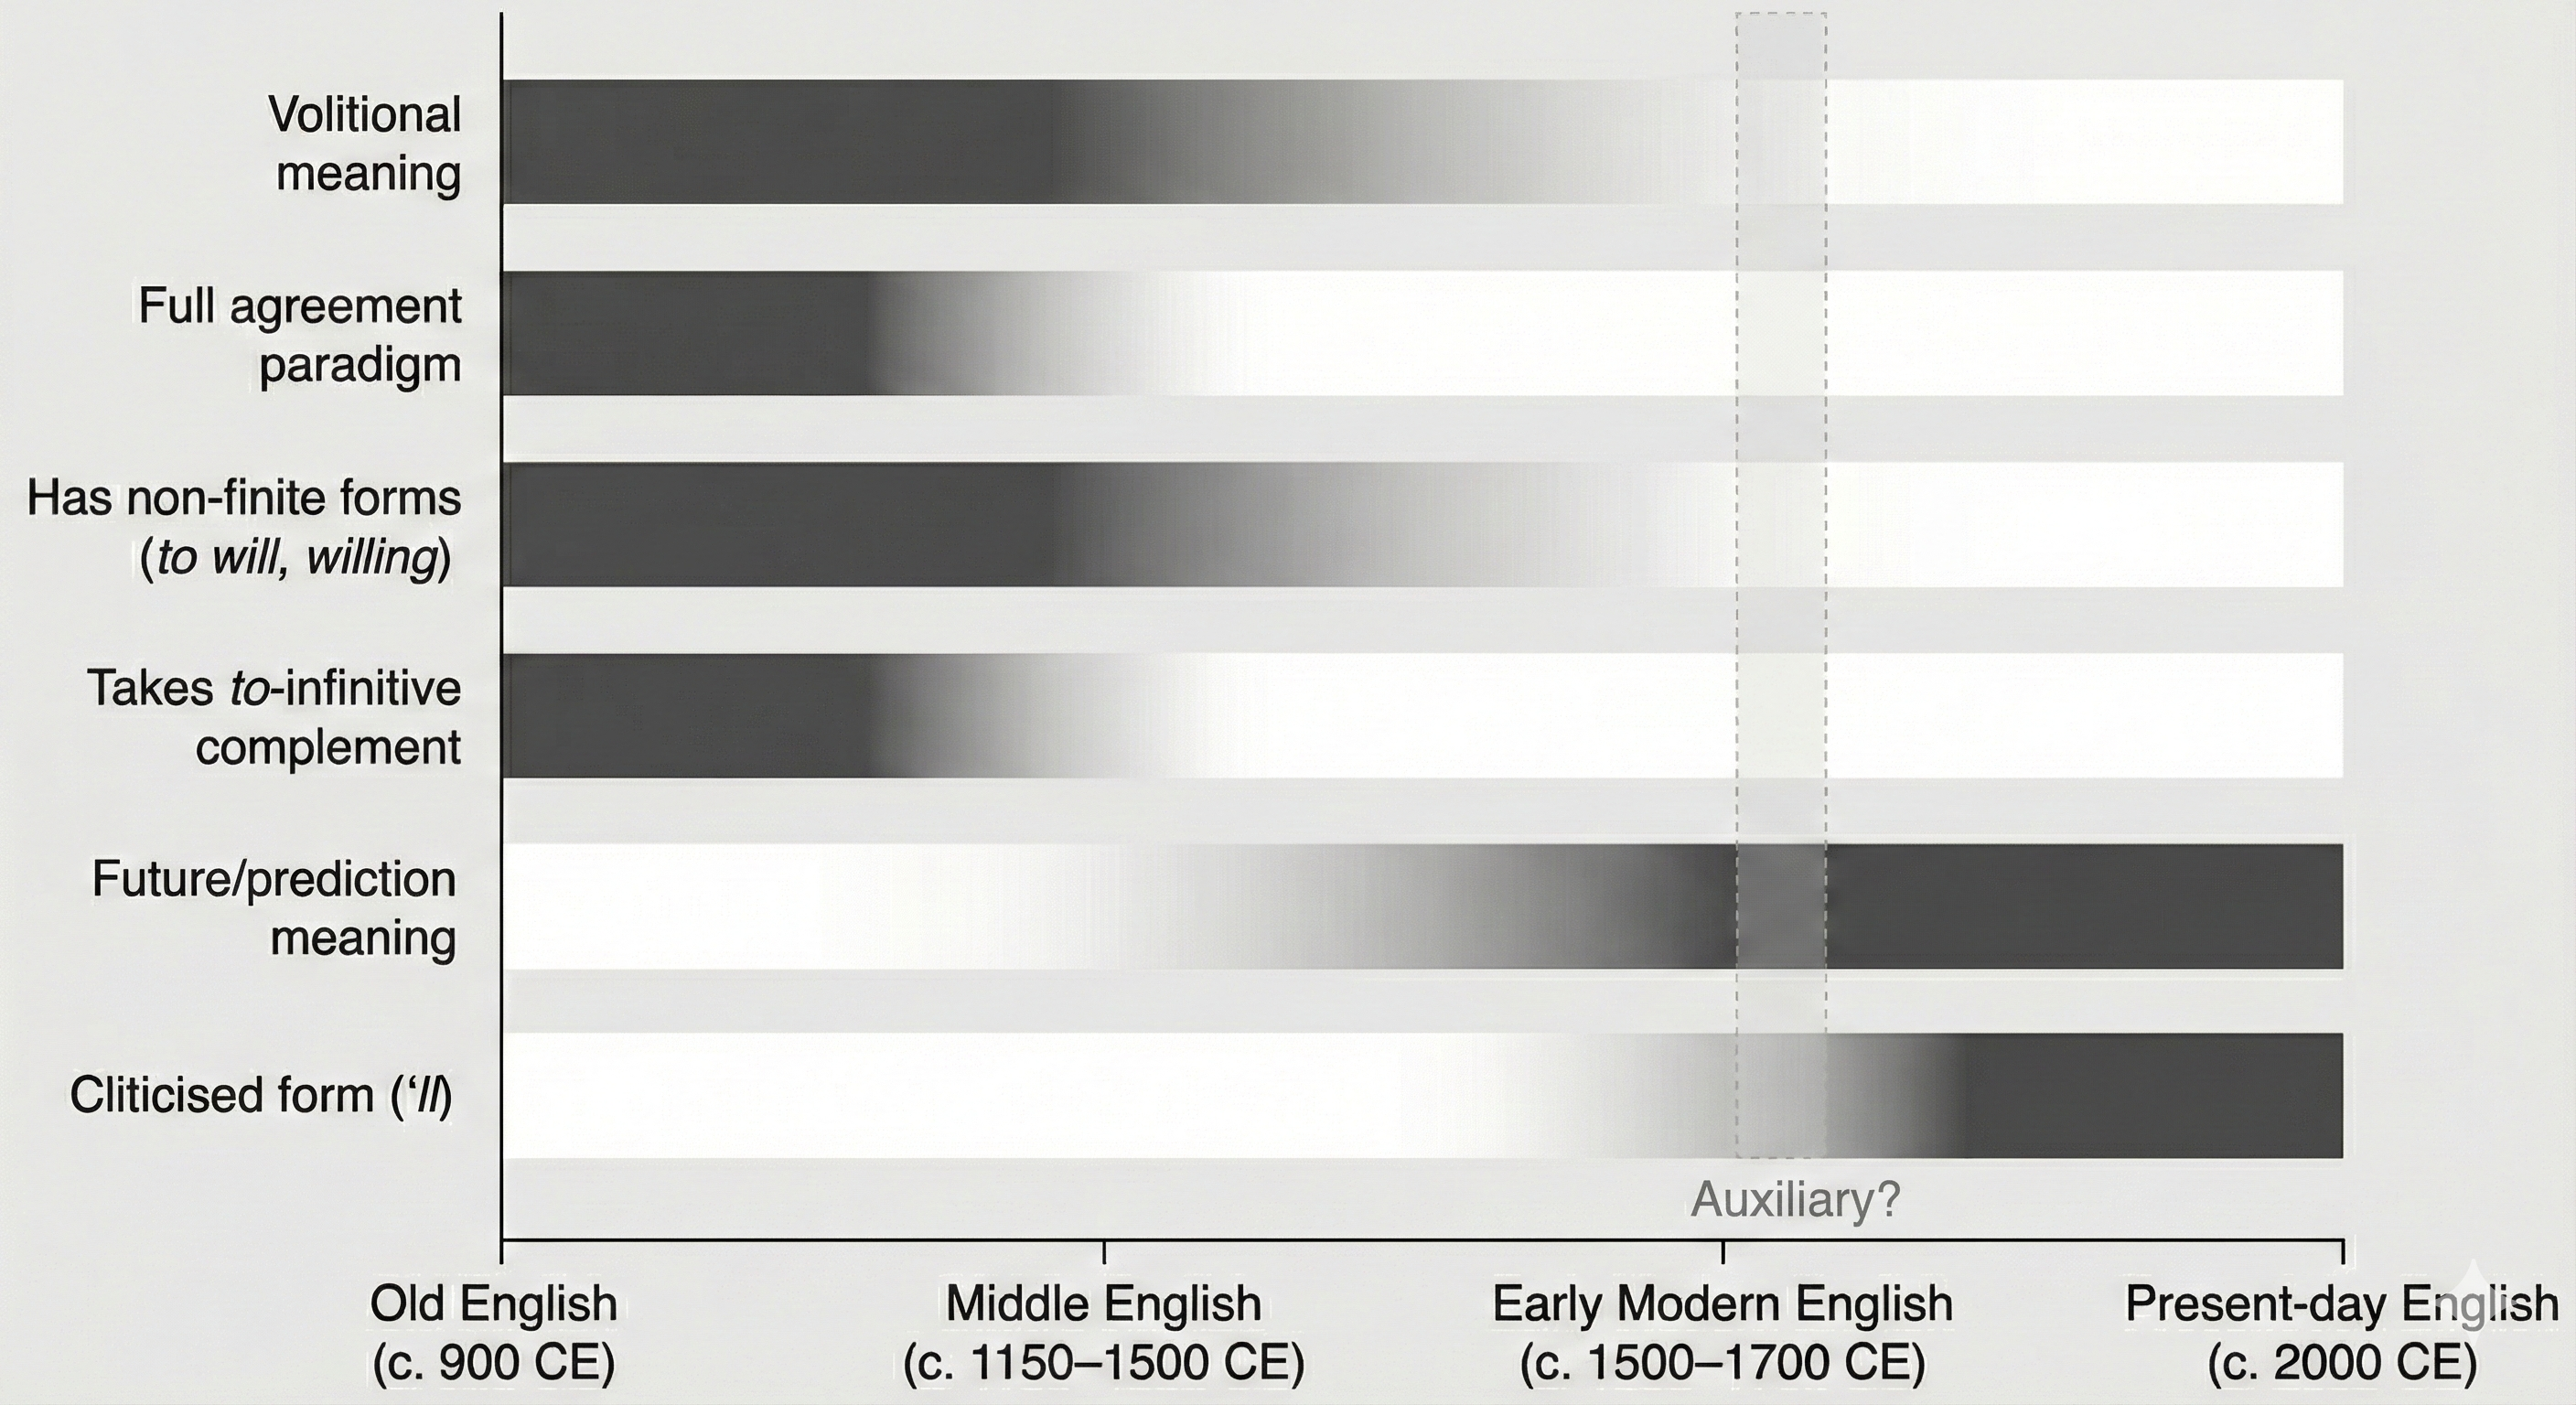
\includegraphics[width=0.9\textwidth]{figures/2.1.png}
    \caption{The grammaticalization of \textit{will}. Lexical-verb properties 
    (volitional meaning, full agreement, \textit{to}-infinitive complements, 
    non-finite forms) fade out gradually; auxiliary properties (future meaning, 
    cliticisation) fade in. The changes are staggered and gradient. Essentialism 
    requires a threshold-crossing moment; the historical record shows a slope.}
    \label{fig:will-trajectory}
\end{figure}

The problem isn't merely epistemological~-- not just that we can't tell when \mention{will} became an auxiliary. The problem is ontological. There's no moment at which \mention{will} became an auxiliary because \mention{becoming an auxiliary} isn't the kind of process that has a moment. It's a gradual shift in a cluster of properties, driven by frequency, phonological reduction, semantic bleaching, analogical extension, and reanalysis by learners. The boundary zone isn't a failure of classification but the mechanism of change itself.

This reframes synchronic boundary cases. Verbless clauses, the classification of \mention{near}, and the disputed \term{subject} constructions in ergative languages~-- these aren't embarrassments to be resolved by finding the right definition. They're snapshots of categories under pressure. Some items are moving into a category; some are moving out; some are stable at the boundary. The boundary zone is populated because language change populates it. Asking \enquote{is this really an X?} presupposes a stable kind for items to be inside or outside of. Grammaticalization shows that the kinds themselves are moving.

The essentialist response is to distinguish synchrony from diachrony. Synchronic grammar describes a static system; diachronic linguistics describes transitions between systems. At any given moment, the categories are fixed; over time, one system replaces another. This preserves essentialism by treating change as external to grammar proper.

But the distinction doesn't hold. If the boundary zone is always populated~-- if, at every synchronic slice, there are items in transition~-- then the static system is a fiction. What looks like a bounded category is a standing wave: apparently stable, dynamically maintained, with continuous flow through the boundary region. The wave is real. Its edges aren't.

Essentialism treats synchrony as primary and diachrony as derivative: change is movement from one state to another, and the states are what have essences. The diachronic evidence inverts this~-- synchrony is slow diachrony, the stability a dynamic equilibrium rather than stasis, and the categories, though real, are processual rather than definitional.

This is another question essentialism can't ask. It can ask: what is the essence of \term{auxiliary}? It can't ask: what mechanisms move items into and out of the auxiliary cluster? The first question has no answer, because there's no essence. The second question has answers~-- frequency effects, phonological reduction, constructional analogy, acquisition biases~-- but the answers are invisible within essentialist framing.

\section{The blocked question}
\label{sec:2:the-blocked-question}

The pattern across these cases isn't just \enquote{definitions fail.} Definitions fail in a specific way that blocks a specific question.

When criteria diverge, essentialism frames the problem as: \textit{Which criterion is correct?} Which property is truly essential to \term{subject}, to phoneme, to clause? The debate becomes a search for the right definition, and because the framework provides no resolution procedure, the search continues indefinitely.

The question that essentialism can't foreground is: \textit{Why do these criteria converge in the first place?} The first question assumes the category and searches for its boundary. The second treats the category itself as the thing to be explained.

For canonical nouns, morphological, syntactic, and semantic criteria all pick out the same set. That isn't a trivial convenience; it's a fact about how linguistic structure is packaged. What keeps those properties bundled together strongly enough that \term{noun} is useful for most of the lexicon? And what happens in the boundary zone where the bundling weakens?

Boundary cases~-- verbless clauses, near-mergers, disputed \term{subject} constructions in ergative languages~-- are where the explanandum becomes visible. Under essentialism they are embarrassments. Outside essentialism they are the natural place to look for whatever keeps the usual alignment intact.

Some traditions have begun asking this second question; Chapter~\ref{ch:what-we-havent-been-asking} surveys what they get right and what they still don't ask.



\begin{figure}[htbp]
    \centering
    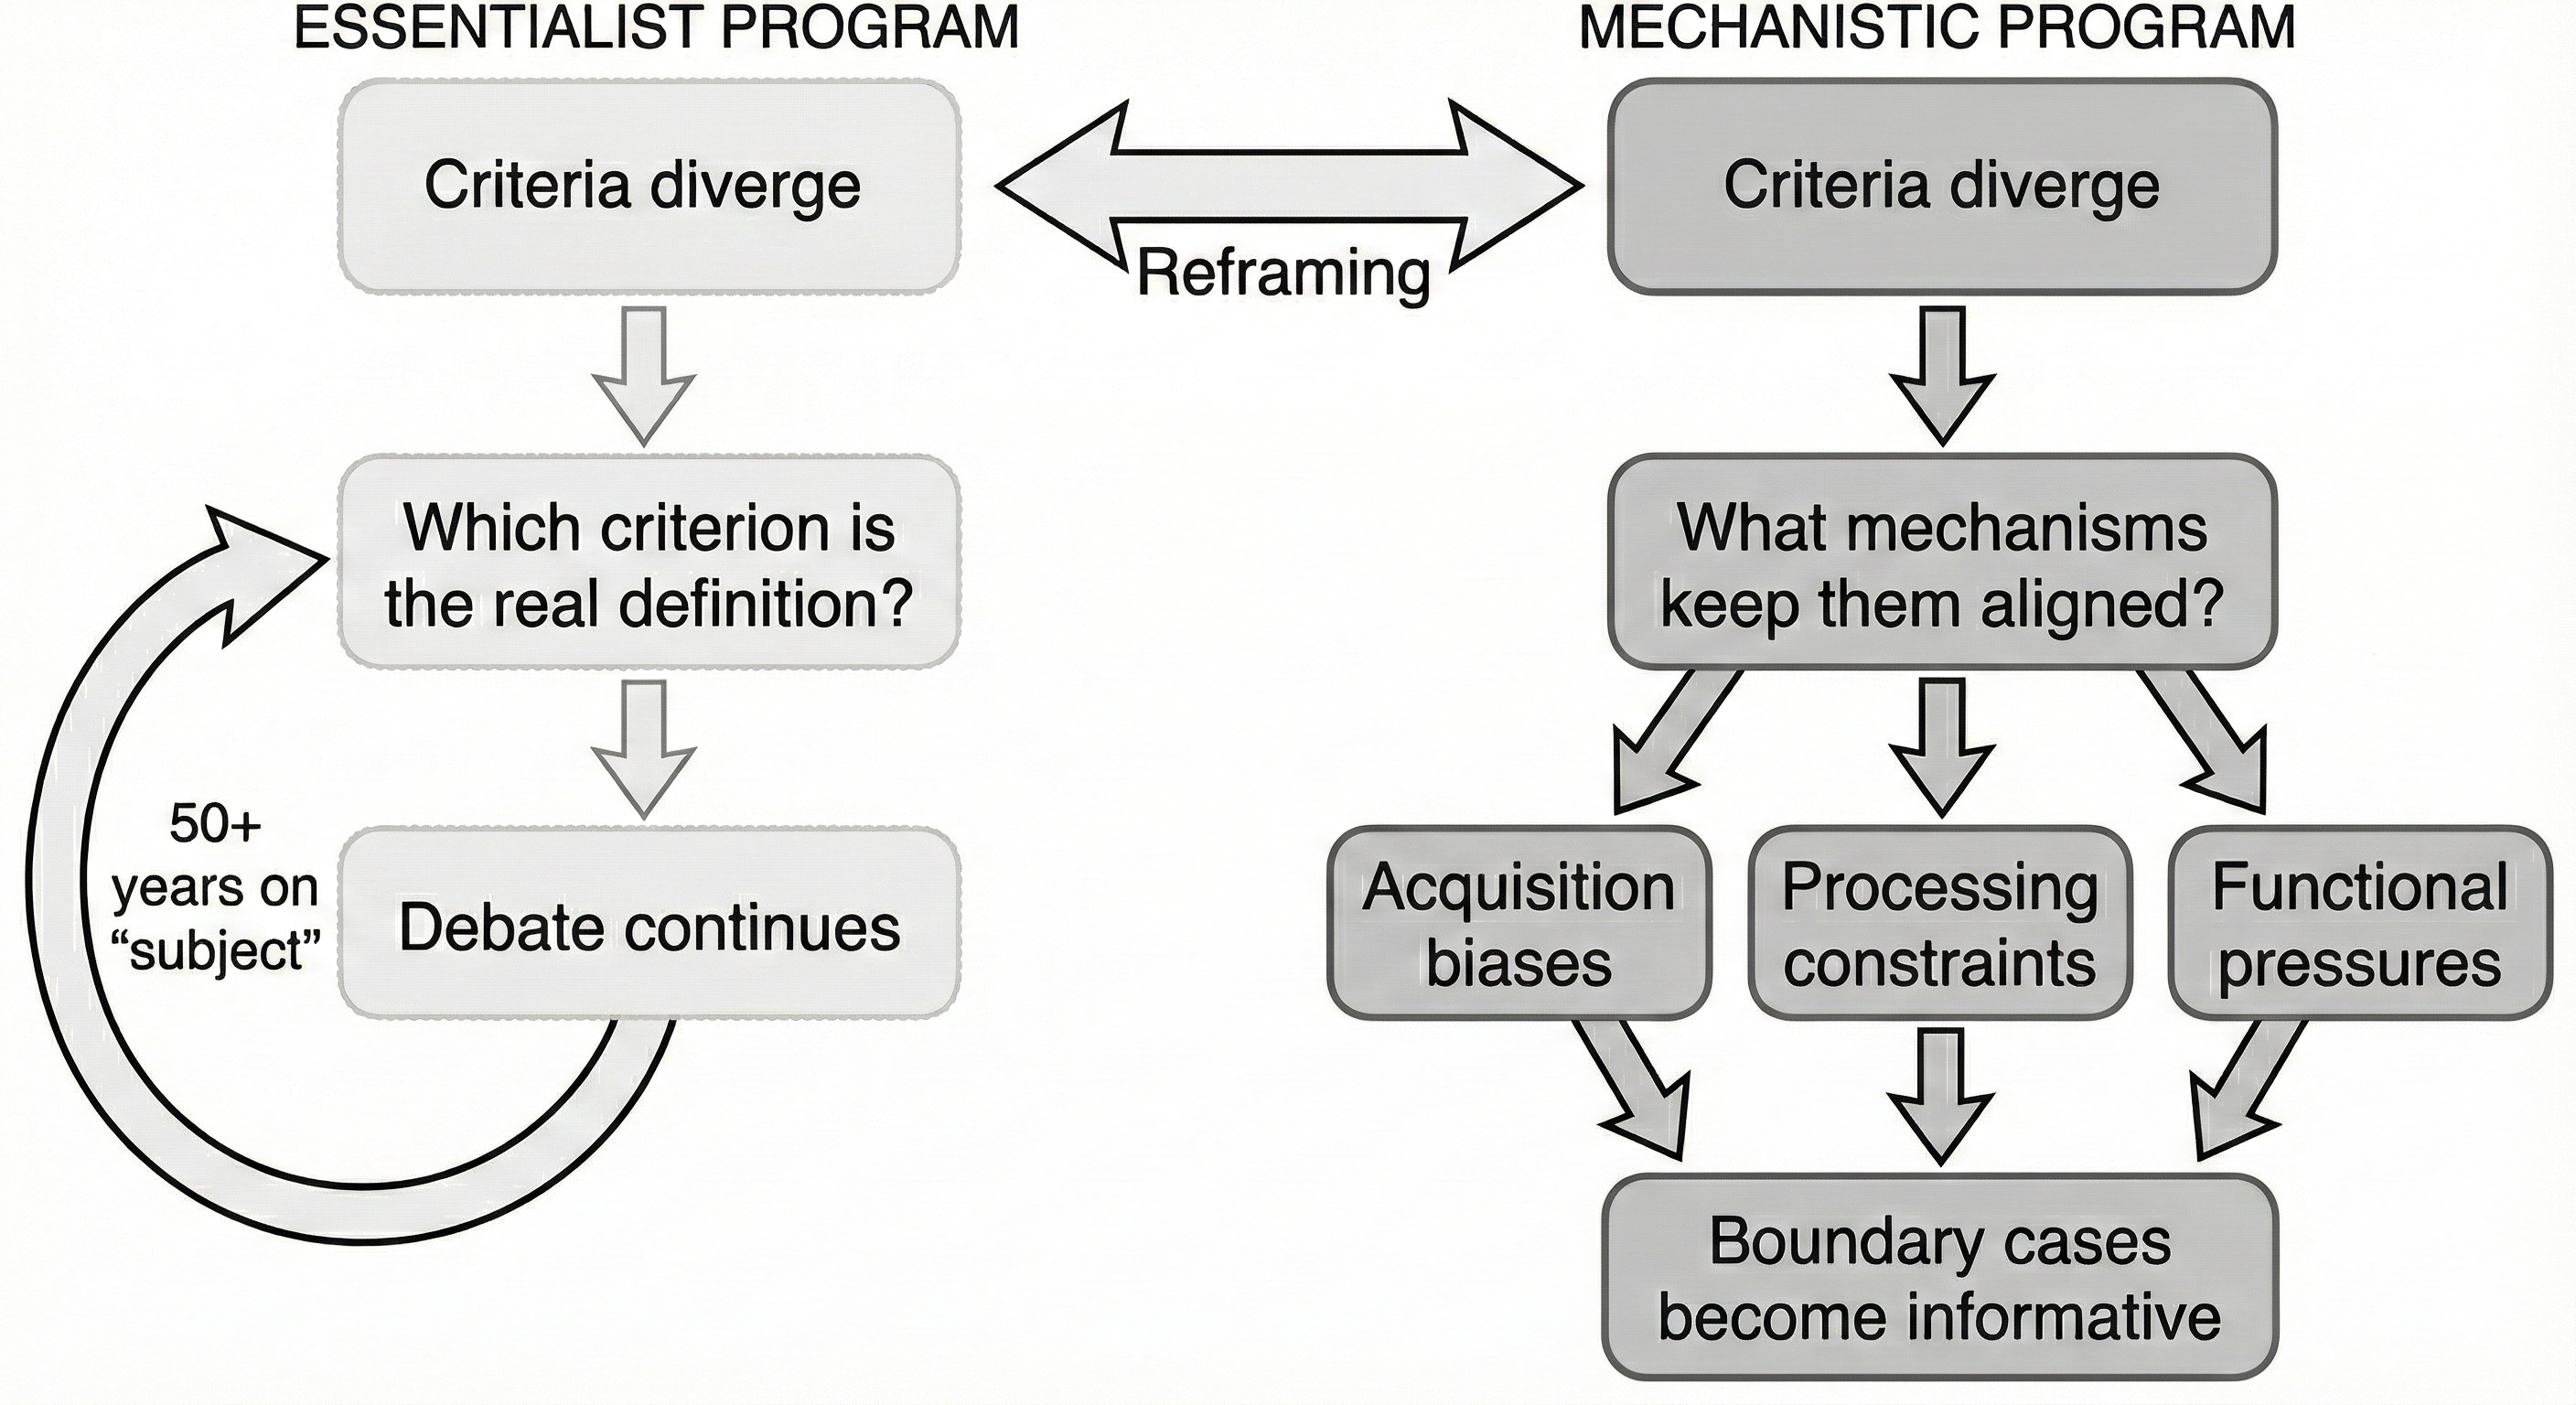
\includegraphics[width=0.75\textwidth]{figures/2.2.png}
    \caption{Two responses to criterion divergence. The essentialist 
    program asks which criterion is definitional and cycles indefinitely. 
    The mechanistic program asks what produces convergence in the first 
    place, transforming boundary cases from embarrassments into evidence.}
    \label{fig:blocked-question}
\end{figure}


\section{A parallel}
\label{sec:2:a-parallel}

This pattern will be familiar to philosophers of biology.

What is a species? For a century, biologists offered criteria: morphological species concepts, biological species concepts \autocite{mayr1942}, phylogenetic species concepts, ecological species concepts. Each is internally coherent. They don't converge on the same groupings. Some populations are connected by gene flow in a geographic ring but reproductively isolated at the endpoints; some hybridize freely; some reproduce without recombination at all. These are the boundary cases~-- ring species, hybrid zones, asexual lineages~-- where criteria come apart and the definitional debate stalls.

The diachronic problem recurs too. Asking at what precise moment a lineage ceased to be a dinosaur and became a bird is like asking when \mention{will} became an auxiliary. The question demands a boundary that the process of evolution doesn't supply.

And morphology can diverge sharply from phylogeny.

\textit{Smilodon} (the sabre-toothed cat) and \textit{Thylacosmilus} (a South American marsupial predator) are separated by over a hundred million years of mammalian evolution (Figure~\ref{fig:convergent-morphology}). They share no recent common ancestor. Yet their skulls are nearly identical: massive canines, robust zygomatic arches, hypercarnivorous dentition. Place them side by side and you see the same animal, arrived at twice.

\begin{figure}[htbp]
    \centering
    \includegraphics[width=0.85\textwidth]{figures/2.3.png}
    \caption{Convergent morphology without shared essence. \textit{Smilodon} 
    (top) and \textit{Thylacosmilus} (bottom) evolved nearly identical 
    skull architecture despite over 100 million years of phylogenetic 
    separation. A morphological species concept groups them; a phylogenetic 
    one separates them. The convergence is explained not by shared ancestry 
    but by similar functional pressures~-- hypercarnivory, ambush predation~-- 
    producing similar solutions \autocite{zimmer2010tangled}. © Carl Buell (image used with permission).}
    \label{fig:convergent-morphology}
\end{figure}

A morphological species concept groups them; a phylogenetic one separates them. The parallel to linguistics is exact: when criteria diverge, essentialism offers no resolution, only continued assertion about which criterion is \enquote{really} definitional. But the convergence itself~-- why these two lineages, under similar selective pressures, evolved nearly identical forms~-- is the phenomenon that demands explanation. Chapter~\ref{ch:kinds-without-essences} will show how mechanistic pressures can explain convergence without requiring shared essence.

For a century, the debate was framed as: which criterion is the correct definition of \term{species}? The debate didn't resolve. It couldn't resolve, because the framework assumed there was an essence to be discovered.

What dissolved the debate wasn't a better definition but a different question. Instead of \enquote{What is a species?} biologists began asking \enquote{What mechanisms maintain this population as a cohesive unit over time?} The answer varies: gene flow, shared selection pressures, developmental constraints, mate recognition systems. Different mechanisms predominate in different cases. \term{Species} names not a single kind defined by a single essence but a cluster of populations maintained~-- flexibly~-- by overlapping mechanisms.

This shift~-- from definition-seeking to mechanism-seeking~-- is what made boundary cases informative. Ring species aren't embarrassments to be explained away; they are evidence of what happens when isolating mechanisms operate incompletely. Hybridization isn't a failure of species boundaries; it reveals the conditions under which reproductive isolation is maintained or breaks down.

Chapter~\ref{ch:kinds-without-essences} will develop this parallel in detail. For now, note only that linguistics isn't alone in facing essentialist failure: the pattern is general, and so, potentially, is the solution.

\section{Why essentialism persists}
\label{sec:2:why-essentialism-persists}

If essentialism fails this reliably, why does it persist?

The persistence has structural causes, and understanding them clarifies what would be needed to shift the field.

Textbooks freeze the architecture. Introductory grammars present categories as checklists: a noun is a word that does X, Y, Z. Students internalise this method before encountering the problem cases that strain it. By the time they reach the boundary phenomena, the framework feels like common sense rather than a theoretical commitment. Pedagogy rewards clean definitions; complexity looks like failure to teach clearly.

Publication norms reward definitional disputes. \textcite{postal1966} titled his paper \enquote{On so-called \enquote{pronouns} in English}~-- scare quotes announcing that pronouns aren't really pronouns but determiners preceding silent nouns. The paper launched decades of debate, culminating in Abney's DP hypothesis \autocite{abney1987}~-- an unpublished dissertation that nonetheless reshaped the field, less through empirical vindication than through perceived endorsement. A paper arguing that X is really Y~-- that raising verbs are really control verbs, that determiners are really functional heads, that the passive is really a species of unaccusativity~-- has a clear contribution: it advances a position in a debate. A paper arguing that the X/Y boundary is gradient and maintained by multiple mechanisms has a murkier contribution. It sounds like giving up. The rhetoric of \enquote{really} signals progress; the rhetoric of \enquote{it depends} signals inconclusiveness. The \enquote{is X really Y} literature could furnish a small library. The library's classification system would be disputed.

Practical applications feed back into theory. Parsers need discrete categories. Corpus annotation schemes need consistent labels. The Penn Treebank~-- the foundational training corpus for a generation of NLP systems~-- collapsed prepositions and subordinating conjunctions into a single tag because annotators couldn't reliably distinguish them; the original Brown Corpus showed inconsistent tagging even in identical syntactic contexts \autocite{marcus1993}. Speech recognition systems need boundaries. The engineering demands are real, and they create pressure to treat categories as if they were determinate even when the theoretical grounds for doing so are shaky. When the parser works, it feels like vindication. When it fails at boundaries, the failure is attributed to noise or insufficient data, not to the ontology. Neural language models~-- especially transformers~-- have loosened this constraint somewhat: they learn distributed representations that can accommodate gradience without requiring sharp categorical boundaries \autocite{vaswani2017attention}. But the theoretical pressure remains. The models are trained on categorically annotated data; the evaluation metrics presuppose discrete labels; the engineering culture inherited essentialist assumptions even as the architectures became more flexible.

Definitions feel like progress. Stating necessary and sufficient conditions feels like achieving something~-- like you've finally said what X \emph{is}. The phenomenology is satisfying in a way that mechanism-talk isn't. \enquote{A clause is a VP-headed structure} is crisp. \enquote{Clausehood is a cluster of properties maintained by functional, acquisitional, and processing pressures that usually but not always co-occur} is accurate but unsatisfying. The crispness is illusory, but illusions can be motivating.

None of this was conspiracy. It's ordinary institutional dynamics. Taken together, textbooks, journals, applications, and definitions form a machine that rewards sharp boundaries, punishes hedging, and naturalises essentialism. The failures are visible only to those already sceptical; the successes are built into the infrastructure that trains the next generation.

The same could be said of any alternative, including the one I'll propose. But explaining why a view persists doesn't settle whether it's true~-- that's determined by whether the framework handles the data. The sociology explains the lag between failure and recognition, not the failure itself.

\section{Conclusion}
\label{sec:2:conclusion}

A final clarification. Nothing in this chapter denies that sentences have structure or that categories are real. The intuition that \textit{The dog bit the man} differs from \textit{The man bit the dog}, and that \textit{dog} and \textit{table} cluster together, is correct. What this chapter denies is the essentialist account of what makes such facts hold.

The choice isn't essence or chaos. If the essentialist says categories are defined, and is wrong, it doesn't follow that categories are arbitrary. Categories may be real but not immutable, revisable but not capricious, stable because something keeps them stable.

The verbless clauses remain. \textit{CGEL}'s definitions are still incoherent. What the incoherence points to isn't the need for better definitions but for a different explanatory target: an account of why the familiar criteria usually line up, and why they sometimes come apart.

But first we need to see what falls out of view when the field tries to escape essentialism's grip~-- whether by retreating to nominalism or by working around the problem with gradience and usage-based mechanisms without quite confronting it head-on.
